\chapter{Computer lower bounds}\label{chap:lb}

% potential todo: why are lower bounds so hard?

In this chapter, we focus on the algorithmic approach to computing
lower bounds for \binstretch. We explain the technique of Gabay,
Brauner and Kotov~\cite{gabay2013lbv2} as well as our extensions and
its implementation.

\paragraph{An intermezzo with an anecdote.} Before we continue with
the explanation of the central ideas of our computer search, let us
pause to explain the motivation of the thesis author to work on the
lower bound algorithms.

While working together with Jiří Sgall, Rob van Stee and Pavel Veselý
on the algorithmic results of Chapters~\ref{chap:manybins} and
\ref{chap:threebins}, we have also investigated lower bounds for
\binstretch. With some effort, the author of this thesis was able to
prove a lower bound of $4/3 + \varepsilon$ for $3$ bins and a very
small value of $\varepsilon$.

To our surprise, another paper on \binstretch appeared while we were
working on the problem, namely the one by Gabay, Brauner and Kotov
\cite{gabay2013lbv2} showing a much better lower bound of $19/14$
using a clever minimax computer search and using a CSP solver to
verify the optimum guarantee in every step. Gabay et al. were able to
check all integer denominators up to $20$, after which their computer
program ran out of memory.

In this paper of Gabay et al. (but unfortunately not in its current,
updated version) we could find the following fateful sentence:

\textit{``The combinatorial explosion is very well illustrated in column
\texttt{\#nodes} where we can see that even with many efficient cuts,
we cannot tackle much larger problems.''}\cite{gabay2013lbv2}

Even though the sentence itself might be considered incorrect (seeing
as we \emph{can} tackle much larger problems, and in fact we will
tackle problems up to denominator $82$), the author of this thesis
considers it quite ingenious. That one sentence turned a reasonably
good result into a challenge and ignited the author's spark for
computer lower bounds.

\section{Minimax algorithm}\label{sec:4:minimax}
Let us recall the bin stretching game, as defined in the introduction:

\begin{dfn}
Fix a number of bins $m$ and a stretching factor $R$. The \emph{bin stretching game}
is defined as follows:

\begin{enumerate}
\item It is a two-player game between \algo and \adversary, and the player \adversary starts.
\item The player \adversary moves by sending any item $i \in (0,1]$ with the restriction
that $i$ along with all previous items can be packed into $m$ bins of capacity $1$.
\item The player \algo moves by selecting a bin where the item is packed.
\end{enumerate}

The winning states are defined thus:
\begin{itemize}
\item A state is winning for \algo if all bins are packed strictly below $R$ and \adversary
has cannot make any further moves.
\item A state is winning for \adversary if one bin has total load at least $R$.
\end{itemize}
\end{dfn}

Our main goal is learning whether there exists an algorithm for
\binstretch with stretching factor strictly below $R$, or whether
every algorithm needs a stretching factor of at least $R$. This
directly corresponds to existence of a winning strategy for the player
\algo or \adversary, respectively.

A ``gold standard'' algorithm for evaluating a given combinatorial
two-player game is the \emph{minimax algorithm}, which we can
summarize as follows:

\begin{algorithm}
\caption{Algorithm \textsc{Minimax}$(s)$ for a state $s$}
% \label{alg:bounded}
\begin{algorithmic}[1]
\State \algorithmicif\ the state is defined as winning for any player, return.
\For{every move $m$ of the current player}
\State Construct the state $t$ by applying the move $m$ to the current state $s$.
\State Run \textsc{Minimax}$(t)$.
\State \algorithmicif\ $t$ is winning for the current player, return.
\EndFor
\State \Return the fact that the state $s$ is winning for the other player.
\end{algorithmic}
\end{algorithm}


As we also mentioned in the introduction, the two main obstacles to
implementing \minimax for \binstretch are the following:

\begin{enumerate}
\item \adversary can send an item of arbitrary  size;
\item \adversary needs to make sure that at any time of the game, an offline
  optimum can pack the items arrived so far into $m$ bins of capacity $1$.
\end{enumerate}

To overcome the first problem, it makes sense to create a sequence of
games based on the granularity of the items that can be packed.  The
second problem increases the complexity of every game turn of the
\adversary, as it needs to run a subroutine to verify the guarantee
for the next item it wishes to place.

\section{Description of the finite game}

We now formulate precisely the scaling parameter and other main
concepts of the game we wish to solve. First of all, for scaling
purposes, we rescale the guaranteed load of the optimum packing from
$1$ in the original definition to $S \in \Nat$. Therefore, if the
algorithm must fill at least one bin to capacity $R$, the lower bound
on the stretching factor will be $R/S$.

Next, we formalize what will be one state of our game:

\begin{dfn}\label{dfn:binconf}
  Assume we fix three integral parameters: $m$ (the number of bins), $R$ (capacity of bins of the algorithm)
and $S$ (size of the optimal bin). Then, we define a \emph{bin configuration} to be a pair
  $(\calL,\calI)$, where
  \begin{compactitem}
    \item $\calL$ is a tuple of $m$ non-negative integers, sorted in descending order. These denoting the current sorted loads of the bins.
    \item $\calI$ is a multiset with ground set $\{1,2,\ldots,S\}$ which contains the items used in the bins.
  \end{compactitem}

  Additionally, for every bin configuration, it must hold:
  \begin{compactitem}
    \item that there exists a packing of items from $\calI$ into $m$ bins with loads exactly in $\calL$;
    \item that there exists a packing of items from $\calI$ into $m$ bins that does not exceed capacity $S$ in any bin.
  \end{compactitem}  
\end{dfn}

To illustrate the definition, consider a bin configuration
$((4,3,2,0),\{1,2,2,3,\})$ -- a situation where four items arrived,
one bin is loaded to size $4$, one to size $3$ and one to size $2$,
leaving one more bin empty. Notice that the bin configuration does not
capture the entire history of the game, but only its current state --
indeed, we do not know in which order the items arrived, or even
whether the bin of size $4$ is filled as an item of size $3$ plus an
item of size $1$, or $2$ plus $2$.

Losing information about history might seem like a bad idea at first,
but it becomes more advantageous later, as it makes caching more
efficient.

It is clear that every bin configuration is a valid state of the game
with \adversary as the next player. We may also observe that the
existence of an online algorithm for \binstretch implies an existence
of an oblivious algorithm with the same stretching factor that has
access only to the current bin configuration $m$ and the incoming item
$i$.

In the following easy observation, we make sure that bin configuration
captures all we need for both players:

\begin{obs} Fix parameters $m$,$R$ and $S$.
\begin{enumerate}
\item There exists a lower bound adversarial strategy for \binstretch if and only if there exists a strategy
that receives a bin configuration and returns the next item in the lower bound.
\item There exists an algorithm for \binstretch if and only if there exists an algorithm which receives
a bin configuration and a new item and returns a new bin configuration where the new item is packed.
\end{enumerate}
\end{obs}
\begin{proof}
\end{proof}
We are now able to formally define the game we investigate:

\begin{dfn}
For a given $m \in \Nat, R \in \Nat$ and $S \in \Nat$, the \emph{bin stretching game} $\Game(m,R,S)$ is the following two-player game:

\begin{enumerate}
\item There are two players named \adversary and \algo. The player \adversary starts.
\item Each turn of the player \adversary is associated with a bin configuration $C = (\calL,\calI)$.
The start of the game is associated with the bin configuration $((0,0,\ldots,0),\emptyset)$.
\item The player \adversary receives a bin configuration $C$. Then,
\adversary selects an integer $i$ such that the multiset $\calI \cup
\{i\}$ can be packed by an offline optimum into $m$ bins of
capacity $S$. The pair $(C,i)$ is then sent to the player \algo.
\item The player \algo receives a pair $(C,i)$. The player \algo has
to pack the item $i$ into the $m$ bins as described in $C$ so that
each bin has load \emph{strictly less than} $R$. \algo then updates the
configuration $C$ into a new bin configuration, denoted $C'$. \algo
then sends $C'$ to the player \adversary.
\item If the player \algo receives a pair $(C,i)$ such that it cannot pack
the item according to the rules, the bin configuration $C$ is won for player \adversary.
\item If the player \adversary has no more items $i$ that it can send from a
configuration $C$, the bin configuration $C$ is won for player \algo.
\end{enumerate}
\end{dfn}

\begin{dfn}
We say that a game $\Game(m,R,S)$ is a \emph{lower bound} if the player
\adversary has a winning strategy when starting from the bin configuration
$((0,0,\ldots,0),\emptyset)$.
\end{dfn}

\section{The sequential algorithm}\label{sec:minimax}

Our implemented algorithm is a parallel, multi computer implementation
of the minimax game search algorithm. We now describe a pseudocode of
its sequential version. The pecularities of our algorithm (caching,
pruning, parallelization) are described in the following sections.

One of the differences between our algorithm and the algorithm of
Gabay et al. \cite{gabay2013lbv2} is that our algorithm makes no use
of alpha-beta pruning -- indeed, as either \algo or \adversary have a
winning strategy from each bin configuration, there is no need to use
this type of pruning.

\begin{algorithm}
\caption{Procedure $\evaladv$}
Input is a bin configuration $C = (\calL, \calI)$.
% \label{alg:bounded}
\begin{algorithmic}[1]
\State \algorithmicif\ the configuration is cached (Section~\ref{sec:4:caching}), \Return the value found in cache.
% \item\label{step:heuristics} Apply \adversary-based heuristics (Section \ref{subsec:heuristics}).
\State Create a list $L$ of items which can be sent as the next step of the player \adversary (Section \ref{subsec:test}).
\For{every item size $i$ in the list $L$}
\State Recurse by running $\evalalg(C,i)$.
\State \algorithmicif\ $\evalalg(C,i)$ returns $0$ (the configuration is winning for player \adversary), stop the cycle and \Return $0$.
\EndFor
% \State \algorithmicelse\ continue with the next item size.
\State \algorithmicif\ the evaluation reaches this step, store the configuration in the cache and \Return $1$ (player \algo wins).

\end{algorithmic}
\end{algorithm}


\begin{algorithm}
\caption{Procedure $\evalalg$}
Input is a bin configuration $C = (\calL,\calI)$ and item $i$.
\begin{algorithmic}[1]
\State Prune the tree using known algorithms (Section \ref{sec:4:gs}).
\For{any one of the $m$ bins}
\If{$i$ can be packed into the bin so that its load is at most $R-1$}
\State Create a configuration $C'$ that corresponds to this packing.
\State Run $\evaladv(C')$.
\State \algorithmicif\ $\evaladv(C')$ returns 1, \Return 1 as well.
\EndIf
\EndFor
\State \algorithmicif\ we reach this step, no placement of $i$ results in victory of \algo; \Return 0.
\end{algorithmic}
\end{algorithm}

\begin{algorithm}
\caption{Procedure $\Sequential$}
\noindent Input is a bin configuration $C = (\calL,\calI)$. 
\begin{algorithmic}[1]
\State Fix parameters $m,R,S$.
\State Run $\evaladv(C)$.
\If{$\evaladv(C)$ returns $1$}
\State \Return failure.
\Else
\State Print the tree currently in memory, erase the bin configuration cache.
\State \algorithmicfor\ any cached bin configuration $C$ that is linked in the tree, run $\Sequential(C)$ with a blank cache.
\State \Return the game tree.
\EndIf
\end{algorithmic}
\end{algorithm}

\newpage
\section{Verifying the offline optimum guarantee}\label{subsec:test}

When we evaluate a turn of the \adversary, we need to create the list
$L = \{0,1,\ldots,y\} \subseteq \{0,1,\ldots,T\}$ of items that
\adversary can actually send while satifying the \binstretch
guarantee. We employ the following steps:

\begin{algorithm}
\caption{Procedure $\MaxFeas$}
\noindent Input is a bin configuration $C = (\calL,\calI)$ with $n$ items and $m$ bins.
\begin{algorithmic}[1]
\State Calculate an upper bound $UB$ on the value $y$.
\State Calculate a lower bound $LB$ on the value $y$ using an online best fit algorithm (Section~\ref{sec:4:dynprogbounds}).
\If{$LB < UB$}
\State Do a linear search on the interval $\{UB,UB-1,\ldots,LB\}$
using a procedure $\Query$($\calI \cup \{i\})$ that queries the cache
whether $\calI \cup \{i\}$ is feasible or not (Section~\ref{sec:4:caching}).
\State Update $LB, UB$ to be the best values confirmed feasible/infeasible by $\Query$.
\EndIf
\If{$LB < UB$}
\State Update $LB$ using the (offline) algorithm \bfd.
\EndIf
\If{$LB < UB$}
\State Compute the exact value of $y$ using a dynamic program $\DynprogMax$ (Section~\ref{sec:4:dynprogmax}).
\EndIf
\State \Return $y = LB = UB$.
\end{algorithmic}
\end{algorithm}

\subsection{Upper and lower bounds}\label{sec:4:dynprogbounds}

If we wish to compute the value $y$ directly, we need to call the
dynamic program $\DynprogMax$, whose complexity is $O(n \cdot S^m)$ in
the worst case (and that is if we ignore potential slowdowns via
hashing).

. This is polynomial when $m$ is a constant, but already
for $m=3$ and especially when $4 \le m \le 9$ such a call per every
game state becomes prohibitively expensive. Therefore we employ
several tricks that help us avoid computing $\DynprogMax$ in some game
states.

First, we compute an upper bound on the maximum feasible item size
$y$.  The upper bound will be $UB \defeq \min(y', m\cdot S - t)$, where
$y'$ is the maximum feasible value that was computed in the previous
vertex of \adversary's turn, and $t$ is the total size of all items i
the instance. The second term is therefore the sum of all items that
can arrive in this instance.

\paragraph{Online Best Fit.} To find the first lower bound quickly, we
employ an online bin packing algorithm \obf. This algorithm maintains
a packing of items $\calI$ to $m$ bins of size $S$ during the
evaluation of the algorithm $\Sequential$, packing each item as it is
selected by the player \adversary. The algorithm \obf packs each item
$i$ into the most-loaded bin where the item fits.

Once the algorithm $\Sequential$ selects a different item $i'$ and
evaluates a different branch of the game tree, the online algorithm
removes $i$ from its bin and inserts $i'$ to the most-loaded bin
where $i'$ fits.

As \obf maintains just one packing, which may not be optimal, it can
happen that \obf is unable to pack the next item $i$ even though $i$
is a feasible item. In that case, we mark the packing as inconsistent
and do not use the lower bound from \obf until its online packing
becomes feasible again.

If the packing maintained by \obf is still feasible, we return as the
lower bound value $LB$ the amount of unused space on the least-loaded
bin.

The main advantage of \obf is that it takes at most $O(m)$ time per
each step, and especially for the earlier stages of the evaluation its
returned value can match the value of $y$.

\paragraph{Checking the cache.} Next, if a gap still remains between
$LB$ and $UB$, we try to tighten it by calling a procedure \Query
which queries the cache of feasible and infeasible item multisets.
The procedure has a ternary answer -- either an item multiset $\calI
\cup \{j\}$ was previously computed to be feasible, or it was computed
to be infeasible, or this item set is not present in the cache at all.

We update $LB$ to be the largest value which is confirmed to be
feasible, and update $UB$ to be $1$ less than the smallest value
confirmed to be infeasible.

\paragraph{Best Fit Decreasing.} If the values $LB$ and $UB$ are still
unequal, we employ a standard offline bin packing algorithm called
\bfd. \bfd takes items from $\calI$ and first sorts them in decreasing
order of their sizes. After that it considers each item one by one in
this order, packing it into a bin where it ``fits best'' -- where it
minimizes the empty space of a bin. We can also interpret it as first
sorting the items in decreasing order and then applying the algorithm
\obf defined above.

As for its complexity, \bfd takes in the worst case $O(m \cdot \calI)$
time. It does not need to sort items in $\calI$, as the internal
representation of $\calI$ keeps the items sorted.

As with \obf, the lower bound $LB$ will updated to the maximum empty
space over all $m$ bins, after \bfd has ended packing. Such an item
can always be sent without invalidating the \binstretch guarantee.

\subsection{Procedure $\DynprogMax$}\label{sec:4:dynprogmax}

Procedure \DynprogMax is a sparse modification of the standard dynamic
programming algorithm for \textsc{Knapsack}. Given a multiset $\calI,
|\calI| = n$ on input, our task is to find the largest item which $y$
which can be packed together with $\calI$ into $m$ bins (knapsacks) of
capacity $S$ each.

% Note that using this formulation it can happen that $|y| = 0$ or even
% that $\calI$ itself is infeasible; however, neither case can happen in
% our actual use of the procedure.

We use a queue-based algorithm that generates a queue $Q_i$ of all
valid $m$-tuples $(a,b,c,\ldots)$ that can arise by packing the first
$i$ items. We do not need to remember where the items are packed, only
the loads of the bins represented by the $m$-tuple.

To generate a queue $Q_{i+1}$, we traverse the old queue $Q_i$ and add
the new item $\calI[i+1]$ to all bins as long as it fits, creating up
to $m$ new tuples that need to be added to $Q_{i+1}$.

Unsurprisingly, we wish to make sure that we do not add the same tuple
several times during one step. We can use an auxiliary $\{0,1\}$ array
for this purpose, but we have ultimately settled on a hash-based
approach.

We use a small array $A$ of $64$-bit integers (of approximately $2^{10} -
2^{13}$ elements). When considering a tuple $t'$ that arises from
adding $i$ to one of the bins in the tuple $t$, we first compute the
hash $h(t')$ of the tuple $t'$. Since we use Zobrist hashing (see
Section~\ref{sec:4:caching}), this operation takes only constant time.

Next, we consider adding $t'$ to the queue $Q_{i+1}$. We use the first
$10-13$ bits of $h(t')$ (let $f$ denote their value) and add $t'$ to
$Q_{i+1}$ when $A[f] \neq h(t')$ -- in other words, when the small
array $A$ contains something other than the hash of $t'$ at the
position $f$. We update $A[f]$ to contain $h(t')$ and continue.

While our hashing technique clearly can lead to duplicate entries in
the queue, note that this does not hurt the correctness of our
algorithm, only its running time in the worst case.

We continue adding new items to the tuples until we do $n$ steps and
all items are packed. In the final pass of the queue, we look at the
empty space $e$ in the least-loaded bin. The output of $\DynprogMax$
and the value of $y$ is the maximum value of $e$ over all tuples in
the final pass.

Ignoring the collisions of the hashing scheme (which can happen but
will not play a big role if we compute the expected running time based
on our randomized hashing function), the time complexity of the
procedure \MaxFeas is quite high in the worst case: $\O(|\calI|\cdot
S^m)$.

Nonetheless, we are convinced that our approach is much faster than
implementing \MaxFeas using integer linear programming or using a CSP
solver (which has been done in \cite{gabay2013lbv2}) and contributes
to the fact that we can solve much larger instances.

\section{Monotonicity}\label{sec:monotonicity}

One of the new heuristics that enables us to go from a lower bound of
$19/14$ on $5$ bins to $9$ bins is iterating on lower bounds by
monotonicity. We define it as follows:

\begin{dfn}
A winning strategy for \adversary has \emph{monotonicity} $k$ if it is true
that for any two items $i,j$ such that $j$ is sent immediately after
$i$, we have $s(j) \ge s(i) - k$.
\end{dfn}

Using this concept, we can iterate over $k$ from $0$ (non-decreasing
instances) to $S-1$ (full generality) to find the smallest value of
monotonicity which leads to a lower bound, if any.

A potential downside of iterating over monotonicity is that it can
introduce a quadratic increase in elapsed time in the case that no
lower bound exists. Additionally, it is quite likely that monotonicity
becomes less useful as the scaling factor $T$ increases, as the item
of relative size $1$ gets smaller and smaller.

Still, solving decision trees of low monotonicity is much faster than
solving the full tree, and we have empirically observed that lower
bounds of lower monotonicity are fairly common; see
Tables~\ref{tab:results3} and \ref{tab:resultsmulti} for our empirical
results.

\paragraph{Monotonicity caveats.} There are two important notes
regarding monotonicity that need to be discussed. First, it is now
true that bin configuration is not enough to describe one state of the
bin stretching game. To see this, consider monotonicity $1$. If the
first three input items are $1,2,3$, the next item needs to be of size
$2$ or larger. However, if the three input items are $1,3,2$ (which is
permissible for monotonicity $1$), the next item on input can be of
size $1$ and above. This means that the two states are not equivalent,
even though their bin configuration is the same.

Notice that this problem is absent in the general case (where any item
can be sent at any time, assuming it satisifies the optimum packing
guarantee) and also in the case of monotonicity $0$ (where the last
item can be inferred from the bin configuration, as it is always the
item with the largest size).

To remedy this, we mark in the bin configuration which item arrived
last in the input sequence, which is sufficient for a fixed value of
the monotonicity. Additionally, we remove all states that are winning
for \algo when switching to the next level of monotonicity, because
these may become winning for \adversary with higher monotonicity.

The second caveat concerns combining other adversarial pruning
(defined later in Section~\ref{sec:advpruning}) with monotonicity.
Since our goal is to quickly find winning strategies for \adversary,
we activate all adversarial pruning tests with all monotonicities,
which means that we may not obey the monotonicity constraints when
using them.

There is no structural problem when doing so, since monotonicity is
only restricting \adversary to reduce the tree size; giving \adversary
some power back is therefore allowed. However, we must take this into
account when reading the results of Tables~\ref{tab:results3} and
\ref{tab:resultsmulti}. For example, a lower bound of monotonicity $1$
may actually allow sending any item in the last few steps of the
instance, provided this leads immediately to \algo packing one
bin fully to its capacity $S$.

\section{Tree pruning}\label{sec:4:pruning}

Alongside the extensive caching described in Subsection
\ref{sec:4:caching}, we also prune some bin configurations where it is
possible to prove that a simple online algorithm is able to finalize
the packing. Such a bin configuration is then clearly won for player
\algo, as it can follow the output of the online algorithm.

\subsection{Algorithmic pruning}\label{sec:4:gs}

Recall that in the game $\Game(m,R,S)$, the player \algo is trying to
pack all items into $m$ bins with load at most $R-1$. If the search
algorithm can quickly deduce that a bin configuration leads to a
successful packing, we can immediately evaluate the configuration as
winning for the player \algo and thus prune the tree.

This may remind us of the \emph{good situations} of
Chapter~\ref{chap:threebins} (specifically Section~\ref{sec:3:gs}).
Indeed, in the case of $3$ bins, we can use the good situations of
Section~\ref{sec:3:gs} directly.

For general $m$, we restate some of the good situations for a general
instance of $\Game(m,R,S)$ such that $(R-1)/S \ge 1/3$. Recall that $\alpha$
is the extra space in a stretched bin; in the situations below, $\alpha = (R-1) -S$,
as the player \algo is packing only to capacity $R-1$.

We omit the proofs of the good situations; they follow the same
arguments as in the proofs in Section~\ref{sec:3:gs}.

\todo{I feel bad for omitting them, but time doesn't seem to be on my side.}

\setcounter{goodsit}{0}

\begin{goodsit}\label{lem:gs1generic}
Given a bin configuration $(\calL,\calI)$ such that the total load
of all but the last bin is at least $(m-1)\cdot S - \alpha$,
there exists an online algorithm that packs all remaining items into
$m$ bins of capacity $R-1$.
\end{goodsit}

\begin{goodsit}\label{lem:gs2generic}
Given a bin configuration $(\calL,\calI)$ such that there exist
two bins $A,B$ such that $s(A) \le \alpha$ and
$s(\calL \setminus \{A,B\}) \ge (m-2)\cdot S - 2\alpha - 1 $,
there exists an online algorithm that packs all remaining items into
$m$ bins of capacity $R-1$.
\end{goodsit}

% \todo{Fix good situations 3 and 4.}

\begin{goodsit}\label{lem:gs3generic}
Consider a bin configuration $(\calL,\calI)$. Define the following
sizes:

\begin{enumerate}
\item Let $s$ be the sum of loads of all bins excluding the last two.
\item Let $r$ (the \emph{last bin load requirement}) be
the smallest load such that if the last bin $B_m$ has load of at least $r$,
GS\ref{lem:gs1generic} is reached.
\item Let $o$ (the \emph{overflow}) be defined as $R-r$.
\end{enumerate}

Then, if $r \le R-1$ and:

\begin{itemize}
\item either the second-to-last bin $B_{m-1}$ has load up to $\alpha$
and above $(m-1)\cdot S - \alpha - o - s$;
\item or the last bin $B_m$ has load up to $\alpha$
bu above $(m-1)\cdot S - \alpha - o - s$;
\end{itemize}

there exists an online algorithm that packs all remaining items into
$m$ bins of capacity $R-1$.
\end{goodsit}

\begin{goodsit}\label{lem:gs4generic}

Suppose that for a bin configuration $(\calL, \calI)$ it holds that
the last two bins are loaded up to $\alpha$. 

Define the following sizes:

\begin{enumerate}
\item Let $r$ be the last bin load requirement as above.
\item Let $c$ (\emph{critical value for $B_{m-1}$}) be equal to $r - s(B_{m-1})$.
(In other words, if an item of size in $[c,S]$ is packed into $B_{m-1}$, GS\ref{lem:gs1generic}
is reached.)
\end{enumerate}

Then, if it is true that for every item size in the interval $[1,c-1]$
we can pack enough of these items into $B_{m}$ such that
$GS\ref{lem:gs1generic}$ is reached on all bins except $B_{m-1}$,
there exists an online algorithm that packs all remaining items into
$m$ bins of capacity $R-1$.

\end{goodsit}

Interestingly, the last good situation (Good Situation
\ref{lem:gs4generic} above) has no fixed threshold like its original
form (GS\ref{lem:gs4}) but is \emph{algorithmic} in the sense that we
can check it for each item size separately with an algorithm and gain
a good situation if all its conditions are met.

\subsection{Adversarial pruning}\label{sec:4:advpruning}

Compared to our fairly strong algorithmic pruning, we have only few
tools to quickly detect that a bin configuration is winning for the
player \adversary. More specificaly, we use only the following two
criteria:

\paragraph{Large item heuristic.} Once any bin has load at least $R-S$,
an item of size $S$ packed into that bin would cause it to reach load
$R$, which is a victory for the player \adversary. Suppose that the
$k$-th bin reaches load $l \ge R-S$. We compute the size of the
smallest item $i$ such that

\begin{enumerate}
\item $s(i) + l \ge R$;
\item For any bin $b$ in the interval $[(k+1), m]$ it holds
that $s(i) + 2l \ge R$; in other words, \algo cannot pack
two items of size $l$ into any bin starting from the $(k+1)$-st.
\end{enumerate}

Finally, we check if \adversary can send $m-k+1$ copies of the item of
size $l$. If so, it is a winning bin configuration for this player and
we prune the tree.

Notice that there may be multiple different values of $l$ for one bin
configuration; for instance, in the setting of $19/14$, for three bins
with loads $11,9,0$, we should check whether we can send $2$ items of
size $10$ or $3$ items of size $8$. Therefore, in the implementation,
we compute for each bin its own candidate value of $l$ and then check
whether at least one is feasible using the dynamic programming test
described in Section~\ref{subsec:test}.

\paragraph{Five/nine heuristic.} We use a specific heuristic for the
case of $19/14$, as it is a good candidate for a general lower
bound. This heuristic was observed to slightly compress the size of
the output tree in this setting.

This heuristic comes into play once there is a bin of load at least
$5$. The item sizes $5$ and $9$ are complementary in the sense that
one of each can fit together in the optimal packing of capacity 14,
but the two of them cannot be packed together into a bin that already
has load at least $5$. Additionally, if there are too many bins of
load at least $5$ but not much more, a subsequent input of several
items of size $14$ will again force a bin of load at least $19$.

We apply this heuristic only when it is true that at all times, $m$
items of size $9$ can arrive on input without breaking the adversarial
guarantee. While this is true, it must be true that all bins are of
load strictly less than $10$.

Our heuristic considers repeatedly sending items of size $5$. If at
any point there are only $p$ bins left with load strictly less than
$5$ and at the same time $p+1$ items of size $14$ can arrive on input,
the configuration is winning for the player \adversary. On the other
hand, if at any point there is a bin of load at least $10$ and the
invariant that $m$ items of size $9$ can still arrive holds, we are
also in a winning state for \adversary.

If it is true that by repeatedly sending items of size $5$ we
eventually reach at least one of the aforementioned two situations,
we mark the initial bin configuration as winning for the player
\adversary.

\paragraph{A note on performance.} While both of our heuristics reduce
the number of tasks in our tree and the number of considered vertices,
we were unable to evaluate them in every single vertex of the game
tree without a performance penalty. Even the large item heuristic,
which can be implemented with just one additional call to the dynamic
programming procedures of Section~\ref{subsec:test} slows the program
down considerably.

This is likely due to the fact that caching outputs of the dynamic
programming calls of Section~\ref{subsec:test} leads to some vertices
that do not need to call any dynamic programming procedure, and with
our heuristics they are forced to call at least one.

We explain the details of our caching strategies in the following
section.

\section{Caching}\label{sec:4:caching}

Our minimax algorithm employs extensive use of caching. We cache
solutions of the dynamic programming procedure \MaxFeas as well as any
evaluated bin configuration $C$ (as a hash) with its value.

\paragraph{Hash table properties.} We store a large hash table of
fixed size with each entry being a 64-bit integer corresponding to
$63$ bits of hash and a binary value. The hash table is addressed
by a prefix of the hash, usually between $20-30$ digits (depending
on the computer used).

We solve the collisions by a simple linear probing scheme of a fixed
length (say $4$). In it, when a value needs to be inserted to an
occupied position, we check the following $4$ slots for an empty space
and we insert the value there, should we find it. If all $4$ slots are
occupied, we replace one value at random.

\paragraph{Hash function.} Our hash function is based on Zobrist
hashing \cite{zobrist}, which we now describe.

For each bin configuration, we count occurences of items, creating
pairs $(i,f)$ belonging to $\{1,\ldots,S\} \times \{0,1\ldots,m\cdot S\}$, where $i$ is the item type
and $f$ its frequency (the number of items of this size packed in all $m$ bins).

For example, we can think of bin configuration
$((3,2,3),\{1,1,1,1,2,3\})$ as a $3$-tuple $(3,2,3)$ along with pairs
$(1,4)$, $(2,1)$, $(3,1)$, $(4,0)$, $(5,0)$ and so on.

At the start of our program, we associate a $64$-bit number with each
pair $(i,f)$. We also associate a $64$-bit number for each possible
load of one bin. These two sets of numbers are stored as a matrix of
size $S \times (m\cdot S)$ and a matrix of size $(R-1) \times m$.

The Zobrist hash function is then simply a \texttt{XOR} of all
associated numbers for a particular bin configuration.

The main advantage of this approach is fast computation of new hash
values.  Suppose that we have a bin configuration $m$ with hash
$H$. After one round of the player \adversary and one round of the
player \algo, a new bin configuration $B'$ is formed, with one new
item placed. Calculating the hash $H'$ of $B'$ can be done in time
$\O(1)$, provided we remember the hash $H$ -- the new hash is
calculated by applying XOR to $H$, the new associated values, and the
previous associated values which have changed.

\paragraph{Caching of the procedure \MaxFeas.} We use essentially the
same approach for caching results in the procedure \MaxFeas, except
only the $m$-tuple of loads needs to be hashed.

We also remark upon the values being cached in the procedure \MaxFeas.
At first glance, it seems that it might be best to store the value of
$y$ with each input multiset $\calI$. However, this is a very bad
idea, as we would lose upon a lot of symmetry.

Indeed, if we set $i$ to be any item from the list $\calI$, we would
lose out on the fact that we know a lower bound on the largest value
that can be sent for a multiset $\calI \setminus \{i\} \cup \{y\}$ --
namely $s(i)$, the value we know is compatible.

Instead, it is much better to cache binary feasibilities or
infeasibilities for a specific multiset $\calI$. We use these results
to improve the values of $LB$ and $UB$ for other calls of procedure
\MaxFeas.

\section{Parallelization}\label{subsec:para}

Up until now, we have implemented a single-threaded minimax algorithm
with caching and pruning. Using this as is, we can improve on the
results of Gabay, Brauner and Kotov \cite{gabay2013lbv2} and reach a
lower bound of $45/33 = 1.\overline{36}$ for $3$ bins and a lower
bound of $19/14$ for up to $5$ bins.

In the pursuit of an improved bound for $3$ bins as well as a general
lower bound for $m$ bins, we have decided to implement a parallel
version of the minimax search algorithm.

\paragraph{Technology.} We have settled on using a combination
of OpenMPI \cite{openmpi} and standard thread library as provided
by the C++ programming language. We have tried implementing


\paragraph{Tasks.} Our evaluation of the game tree proceeds in the
following way: First, we start evaluating the game tree on the main
computer (which we internally call \emph{queen}) until a vertex
corresponding to \adversary's next move meets a certain threshold (for
instance, sufficient depth). After that, we designate this adversarial
vertex as a \emph{task}.

Alongside the queen, we have processes whose job is to evaluate the
tasks -- we call them the \emph{workers}. Workers which run on the
same machine will have a common cache that they access via atomic
primitives in order to maintain consistency. Workers on separate
machines do not share information.

Due to the mixed environment of standard Unix threads and MPI
processes, we also have a single \emph{overseer} per each physical
machine. This overseer handles the MPI communication as well as
spawning the individual worker threads.

The tasks are all generated in advance by the queen. After that, their
bin configurations are synchronized with all overseers running. The
queen then assign tasks to overseers online, namely by assigning a
batch of 250-500 tasks to an overseer. The overseer reports each value
of a finished task immediately to the queen. When an overseer is
finished processing a batch, it requests and receives a new one.

We have selected this communication strategy for two reasons:

\begin{enumerate}
\item To minimize congestion in the processing phase through the fact
that the bin configurations are synchronized beforehand and only
identifiers are shared in the online assignment phase.
\item To allow the queen to evaluate and prune unfinished tasks and
therefore avoid some unnecessary processing by the workers.
\end{enumerate}

\paragraph{Task selection.}
\todo{Finish this paragraph.}

\paragraph{Saplings.} Our implementation also allows us to pre-select
some initial strategy for the player \adversary in advance. This way
we can use our (so far limited) intuitive understanding of what is a
good initial move and decrease the time needed to evalate the whole
tree.

A particularly good strategy for the lower bound of $19/14$ seems to
be sending an item of size $5$ as the first item, followed by $m-1$
items of size $1$. This adversarial strategy leads to a lower bound
instance for $6,7,8$ and $9$ bins.

\todo{Finish this paragraph.}


\section{Results}\label{sec:results}

Table \ref{table:results} summarizes our results. The paper of Gabay, Brauner
and Kotov \cite{gabay2013lbv2} contains results up to the denominator 20; we
include them in the table for completeness. Results after the denominator 20 are
new. Note that there may be a lower bound of size $56/41$ even though
none was found with this denominator; for instance, some lower bound
may reach $56/41$ using item sizes that are not multiples of $1/41$.

\begin{table}
\begin{center}
% \begin{tabular}{ c | @{\hskip 2em} l | @{\hskip 2em} l | @{\hskip 2em} l }\label{tab:results}
\begin{tabular}{ llllll }\label{tab:results3}
 & & & &  \multicolumn{2}{c}{\textit{Elapsed time}}  \\
\textit{Fraction} & \textit{Decimal} & \textit{L. b.} & \textit{Mon.} & \textit{Linear} & \textit{Parallel}\\

\hline
$19/14$ &  $1.3571$ & Yes & 0 & 2s. & \\
$22/16$ & $1.375$ & No & & 2s. & \\
$26/19$ & $1.3684$ & No & & 3s. & \\
\hline
$30/22$ & $1.\overline{36}$ & No & & 6s. & \\
$33/24$ & $1.375$ & No & & 5s. & \\
$34/25$ & $1.36$ & \textbf{Yes} & 1 & 15s. & \\
$45/33$ & $1.\overline{36}$ & \textbf{Yes} & 1 & 1min. 48s. & \\
$55/40$ & $1.375$ & No & & 3min. 6s. & \\
$56/41$ & $1.3659$ & No & & 30min. & 7s. \\
$86/63$ & $1.36507$ & \textbf{Yes} & 6 & & 29s. \\
$112/82$ & $1.3659$ & \textbf{Yes} & 8 & & 3h. 21m. 31s.\\
\end{tabular}
\end{center}
\caption[LoF entry]{The results and performance of our linear and
parallel computations for \binstretch with three bins. The results
above vertical line were previously shown in \cite{gabay2013lbv2}, the
rest are our results. The column \textit{L. b.} indicates whether a
lower bound was found when starting with the given stretching factor
$R/S$ as seen in column \textit{Fraction}.

The column \textit{Mon.} shows the lowest monotonicity that our
program needs to find a lower bound. In the case of negative results,
time measurements were done only using full generality, i.e. with
monotonicity $S-1$.

Some fractions below $112/82$ are omitted; our lower bound computation
has not found a lower bound on those.

The linear results were computed on a server with an AMD Opteron 6134
CPU and 64496 MB RAM. The size of the hash table was set to $2^{25}$
with chain length $4$.

The parallel results were computed using OpenMPI on a heterogenous
cluster with $109$ worker processes running.

The output of the program was not generated during the
time measurements.}\label{table:results}

\end{table}

\begin{table}
\begin{center}
\begin{tabular}{lllllll}\label{tab:resultsmulti}
& & & & & \multicolumn{2}{c}{\textit{Elapsed time}}  \\
\textit{Bins} & \textit{Fraction} & \textit{Decimal} & \textit{L. b.} & \textit{Mon. (5)} & \textit{Linear} & \textit{Parallel (5)}\\
\hline
$4$  & $19/14$ &  $1.3571$ & \textbf{Yes} & & & 18s.  \\
$4$  & $30/24$ & $1.\overline{36}$ & No   & & & 19s. \\
$4$  & $34/25$ &  $1.36$   & No           & & & 48s.  \\ 
$5$  & $19/14$ &  $1.3571$ & \textbf{Yes} & 2 (1) & & 10s. \\
$6$  & $19/14$ &  $1.3571$ & \textbf{Yes} & 0 (0) & & 11s. \\
$7$  & $19/14$ &  $1.3571$ & \textbf{Yes} & 1 (0) & & 2m. 13s. (16s.) \\
$8$  & $19/14$ &  $1.3571$ & \textbf{Yes} & Unk. (1) & & (1h. 14s.)  \\
$9$  & $19/14$ &  $1.3571$ & \textbf{Yes} & Unk. (1) & &  \\
\end{tabular}
\end{center}
\caption{Results produced by our minimax algorithm in the case of $4$
and $5$ bins.  Tested on the same machine and with the same parameters
as in Table~\ref{table:results}, both for linear and parallel
computations. In columns \textit{Mon.} and \textit{Parallel}, we list
in brackets monotonicity and elapsed time of computation for an input
having an item of size 5 at the start. Monotonicity is measured only
starting with the second item.}
\end{table}


\section{Lower bound instance}

This section contains an explicit graphical representation of the
lower bound of $45/33$ for $3$ bins.

\begin{figure}
  \centering
  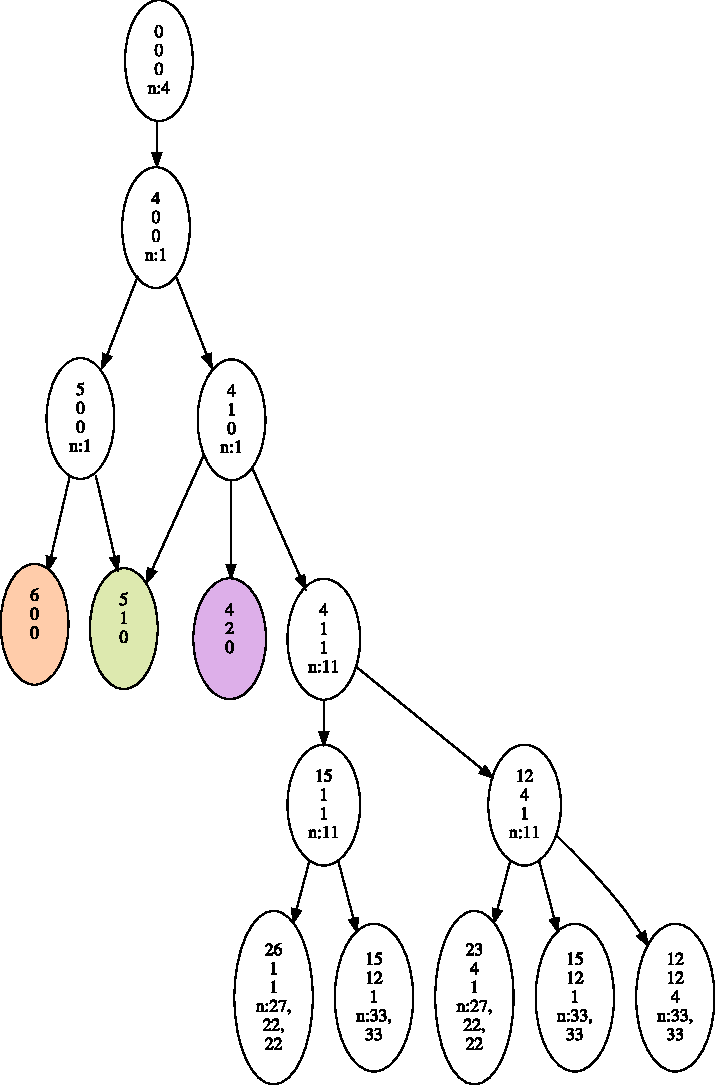
\includegraphics[scale=0.65]{img/big_picture.pdf}
  \caption{The beginning moves of the $45/33$ lower bound, scaled so
      that $T = 33$ and $S = 45$. The vertices contain the current
      loads of all three bins, and a string \texttt{n: $i$} with $i$
      being the next item presented by the \adversary. If there are
      several numbers after \texttt{n:}, the items are presented in
      the given order, regardless of packing by the player \algo. The coloured vertices are expanded in later figures.}
\end{figure}
\newpage
\begin{figure}
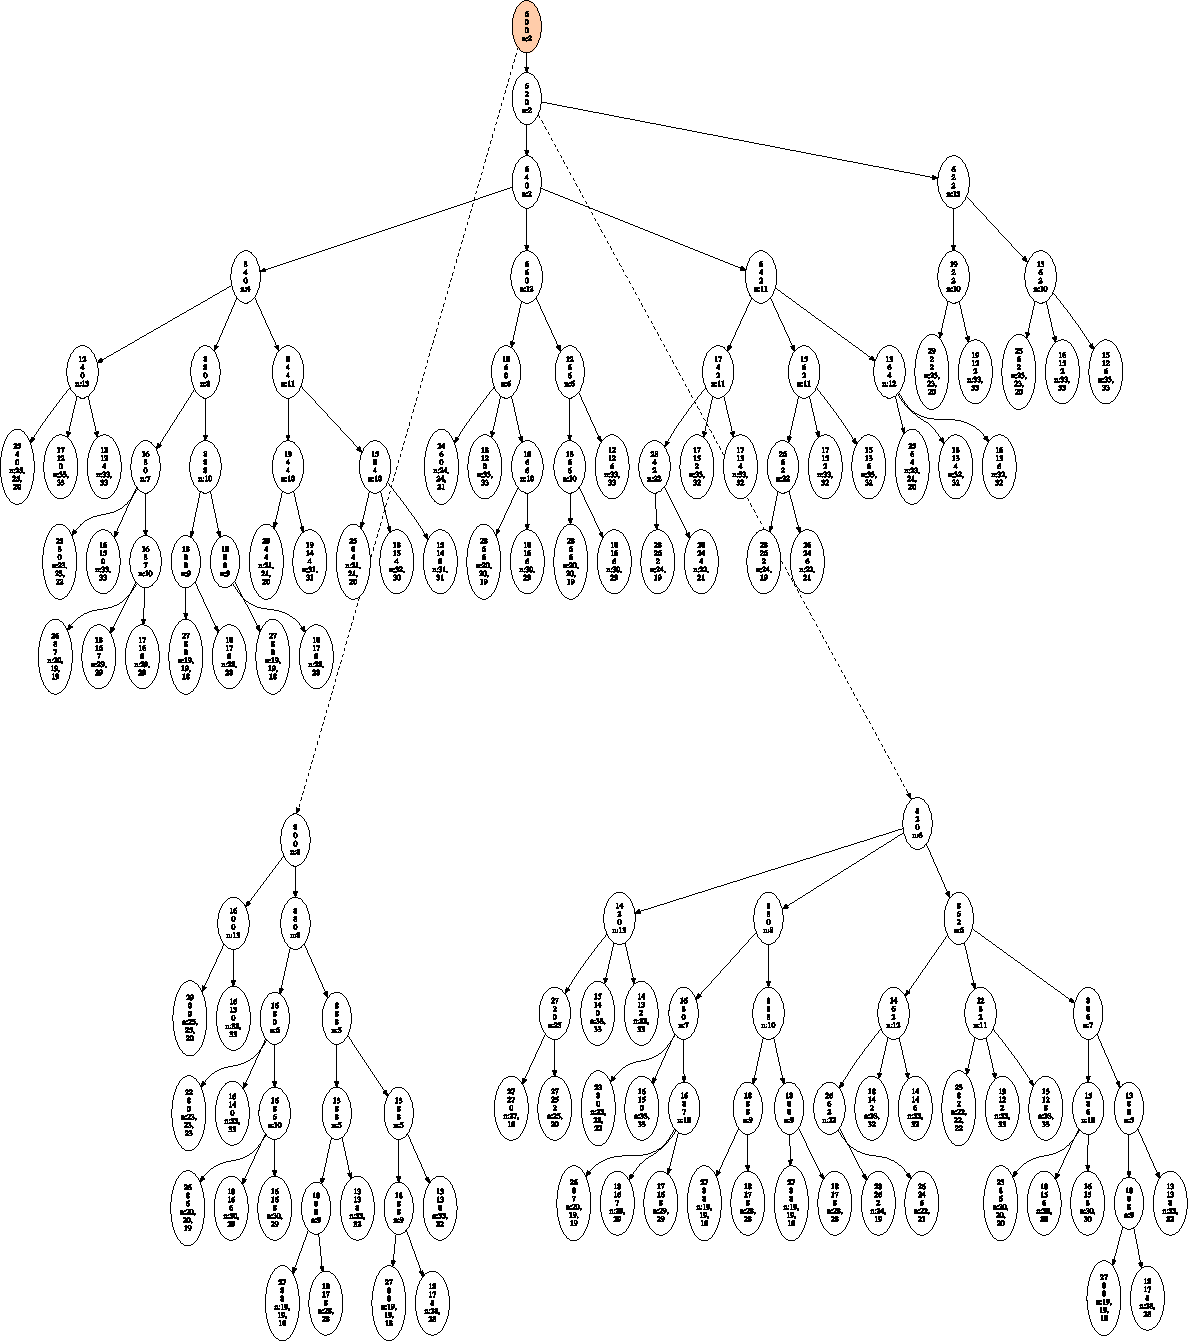
\includegraphics[scale=0.6]{img/6-0-0.pdf}
\caption{Game tree for the lower bound of $45/33$, starting with the bin configuration $(6,0,0,\{4,1,1\})$.}
\end{figure}

\begin{figure}
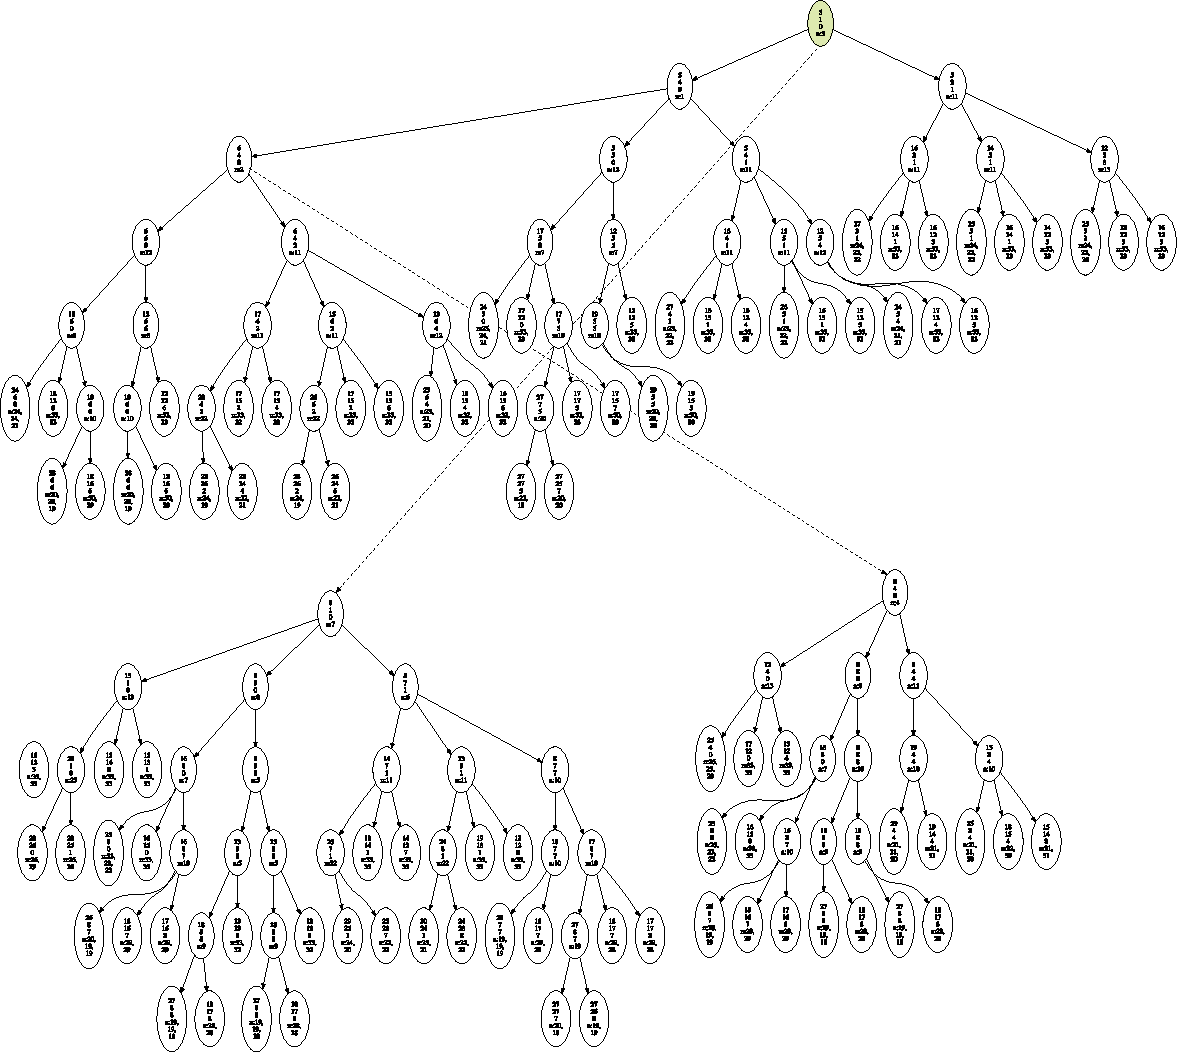
\includegraphics[scale=0.6]{img/5-1-0.pdf}
\caption{Game tree for the lower bound of $45/33$, starting with the bin configuration $(5,1,0,\{4,1,1\})$.}
\end{figure}

\begin{figure}
  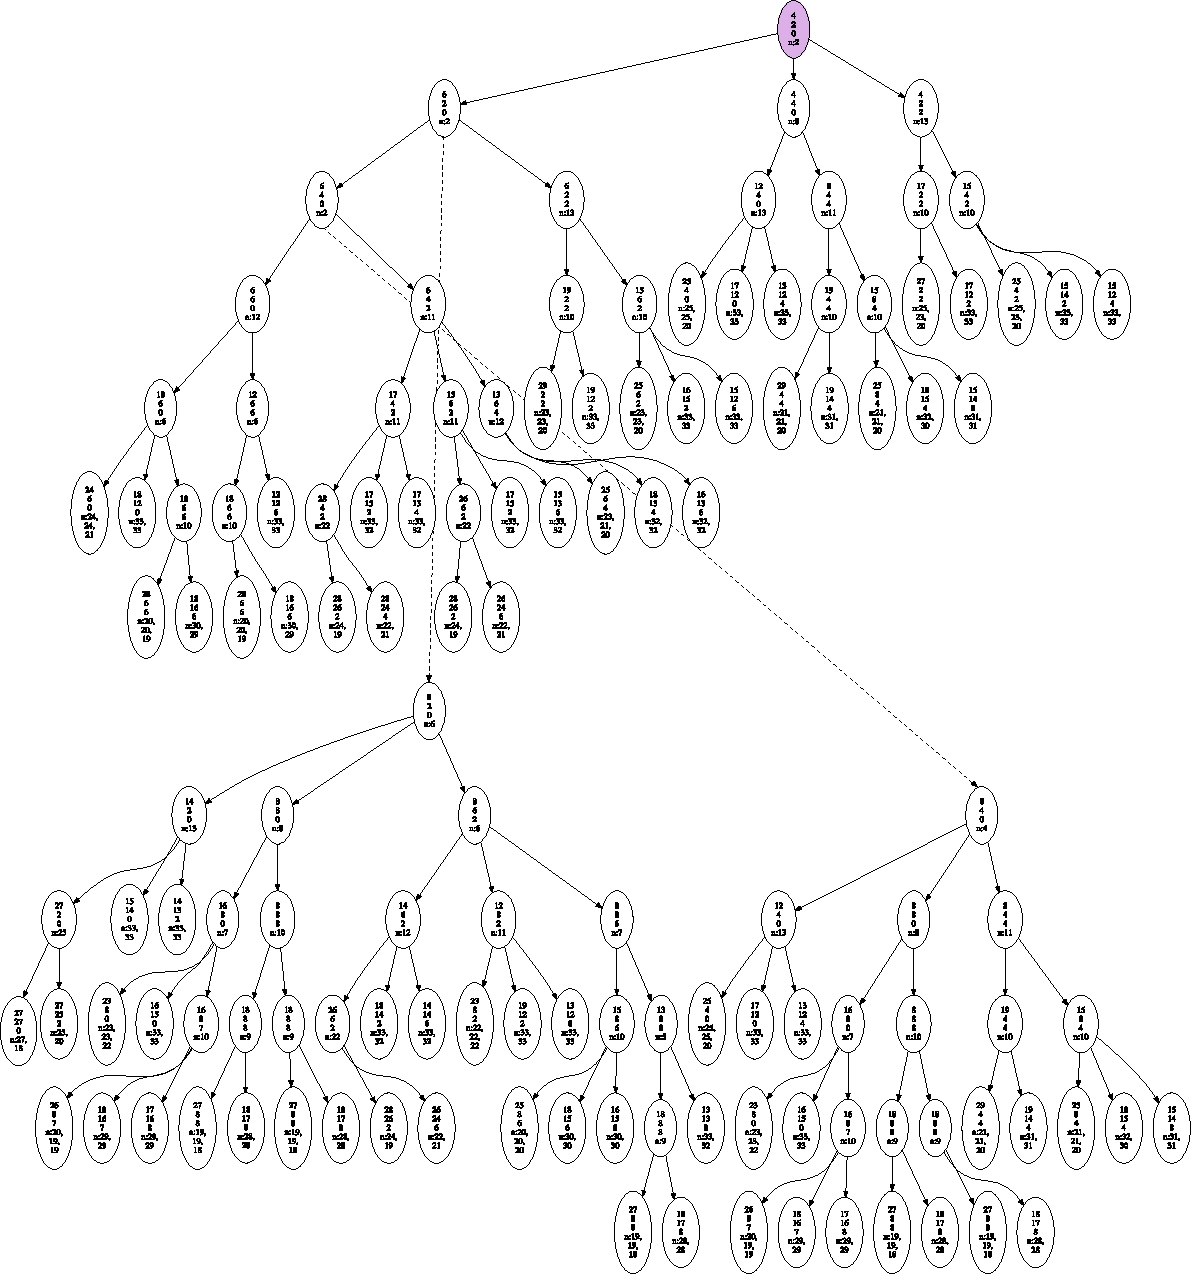
\includegraphics[scale=0.6]{img/4-2-0.pdf}
  \caption{Game tree for the lower bound of $45/33$, starting with the bin configuration $(4,2,0,\{4,1,1\})$.}
\end{figure}

\section{Verification of the results}\label{sec:verification}

\todo{Rewrite this.}

We give a compact representation of our game tree for the lower bound
of $45/33$ for $m=3$, which can be found in Appendix
\ref{sec:appendix}. The fully expanded representation, as given by our
algorithm, is a tree on 11053 vertices.

%TODO: exact number of vertices
For our lower bounds of $19/14$ for $m=4$ and $m=5$, the sheer size of
the tree (e.g. 4665 vertices for a compact representation for $m = 5$) prevents us from
presenting the game tree in its entirety.

We include the lower bound along with the implementations, publishing
it online at
\url{https://github.com/bohm/binstretch/}.

We have implemented a simple independent C++ program which verifies
that a given game tree is valid and accurate. While verifying our
lower bound manually may be laborious, verifying the correctness of
the C++ program should be manageable. The verifier is available along
with the rest of the programs and data.